\documentclass[12pt]{article}
\usepackage[pdftex]{graphicx}
% and their extensions so you won't have to specify these with
% every instance of \includegraphics
\DeclareGraphicsExtensions{.pdf,.jpeg,.png}
\usepackage{url}

\newcommand{\psykal}{{PS}y{KA}l}

\begin{document}

\title{Analysing the Performance of Shallow-Water Models with the
 Roofline Model}

\author{A.~.R.~Porter and R.~W.~Ford}

\maketitle

\section{Introduction}

We want to use the Roofline Model to establish the efficiency (or
otherwise) of two shallow-water benchmark codes that we have used in
the GOcean project.

Although we have investigated how the performance of the \psykal
version of nemolite2d compares with that or the original, we have not
addressed how efficient the original actually is. In order to do so we
use the Roofline Model~\cite{roofline} which provides a relatively
simple way of characterising the performance of a code in terms of
whether it is memory-bandwidth bound or compute bound.

\section{Hardware Details}

In applying the roofline model we follow the approach suggested
in~\cite{para_pearls} and use the well-known STREAM~\cite{stream} and
LINPACK~\cite{linpack} benchmarks in order to get the upper bounds on
the memory bandwidth and FLOPS for the test hardware. Since we are
using Intel CPUs we used the Intel Math Kernel Library
implementation of LINPACK.

\begin{table}
\begin{tabular}{l|c|c|c|c}
  & \multicolumn{2}{c|}{E5-1620 v.~2, 3.7GHz} & \multicolumn{2}{c}{E5-2697 v.~2, 2.7GHz}  \\
  \hline
  L2 Cache (KB)             & \multicolumn{2}{c|}{256} &  \multicolumn{2}{c}{256}  \\
  L3 Cache (MB)             & \multicolumn{2}{c|}{10}  &  \multicolumn{2}{c}{30}  \\
  \hline
  Array size ($10^6$ words) &   0.25 &  5      &  0.25  & 0.5    & 15 \\
  STREAM, Triad (GB/s)      &  35.49 & 17.64   & 29.271 & 13.8426 & 9.6218 \\
  \hline
 LINPACK (GFLOPS)      & \multicolumn{2}{c|}{28.32}  & \multicolumn{2}{c}{25.41} \\
\hline
\end{tabular}
\caption{The STREAM and LINPACK benchmark results for a single thread
  running on each of the two CPUs considered here.}
\label{TAB_stream_linpack}
\end{table}

\section{Hardware Performance Counters}

The likwid tool (\url{https://github.com/RRZE-HPC/likwid}) gives
access to Hardware Performance Counters (HWPCs) on Intel and AMD CPUs.
However, there are issues with the accuracy of these counters,
especially for FLOP-related measurements on Ivybridge architectures. A
tool is included in the likwid distribution that tests the accuracy of
HWPC-derived data by running micro-benchmarks for which the FLOP count
and memory traffic are known:
\url{https://code.google.com/p/likwid/wiki/IvyBridgeVerification}.
The results of doing this on an Intel Xeon E5-1620 v2 CPU are shown in
Figures~\ref{FIG_flops_dp_stream_test}
and~\ref{FIG_flops_dp_triad_test}. It appears that once the memory
footprint spills out of L1 cache (which all of our nemolite2d
benchmark configurations do), the performance counter results
significantly overestimate the FLOPs performed.

\begin{figure}
\centering
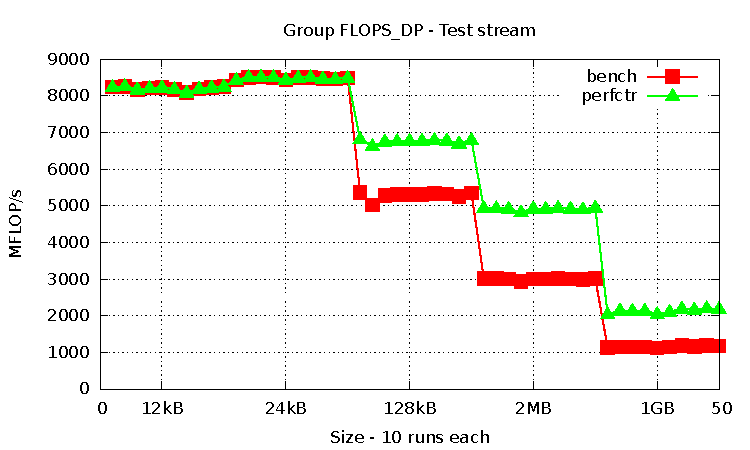
\includegraphics[width=120mm]{FLOPS_DP_stream_ivybridgeEP.pdf}
\caption{Results of the likwid accuracy test for the FLOPS\_DP group
  and the stream benchmark on an Intel Xeon E5-1620 v2.}
\label{FIG_flops_dp_stream_test}
\end{figure}

\begin{figure}
\centering
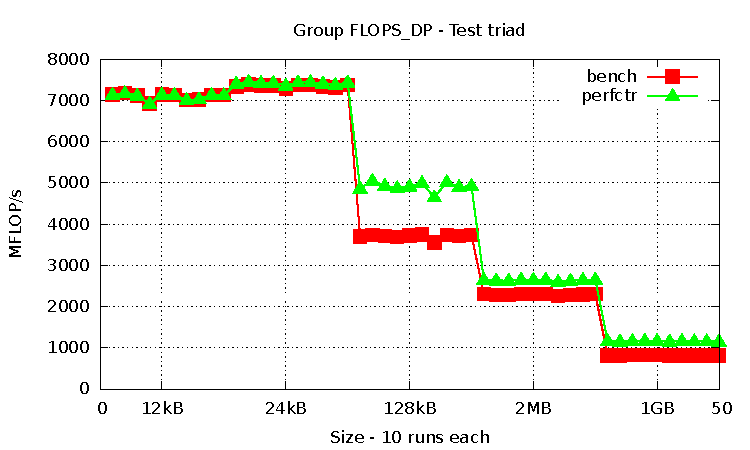
\includegraphics[width=120mm]{FLOPS_DP_triad_ivybridgeEP.pdf}
\caption{Results of the likwid accuracy test for the FLOPS\_DP group
  and the triad benchmark on an Intel Xeon E5-1620 v2.}
\label{FIG_flops_dp_triad_test}
\end{figure}

We therefore need some other way of measuring FLOPS. We could use
likwid on an older Intel CPU (to which we have root access) or try
another tool on the IvybridgeEP system. Other possible tools include
Intel's VTune or OProfile.

\section{Performance Analysis with the Roofline Model}

\subsection{Calculating Kernel Characteristics}

Although the Continuity kernel is very simple, the u-Momentum kernel
is not and in particular, includes a call to the {\tt sin()} function.
In order to estimate the cost of this function in FLOPs the following
code was compiled (with the Intel compiler and -O1) and run with
likwid-perfctr:
\begin{verbatim}
  my_sum = 0.0d0
  do i = 1, 1000
    my_sum = my_sum + sin(real(i))
  end do
  write (*,*) 'My sum = ', my_sum
\end{verbatim}
This measurement revealed that the {\tt sin()} function requires
approximately 13 FLOPs.

A key component of the Roofline model is the Arithmetic Intensity of
the code being executed:
\begin{equation}
AI = \frac{\textrm{No. of floating-point operations}}{\textrm{Bytes fetched from memory}}
\end{equation}
We calculated this quantity manually by examining the
source code and counting the number of memory references and
arithmetic operations that it contained. In doing this counting we
assume that any references to adjacent array elements are fetched in a
single cache-line and thus only count once.

To illustrate this, we consider the first loop-nest in the
time-stepping section of the Shallow code. This is a doubly-nested
loop over {\tt i} and {\tt j} with {\tt i} innermost). The body of the
loop is:
\begin{verbatim}
CU(I+1,J) = .5d0*(P(I+1,J)+P(I,J))*U(I+1,J)
CV(I,J+1) = .5d0*(P(I,J+1)+P(I,J))*V(I,J+1)
Z(I+1,J+1) =(FSDX*(V(I+1,J+1)-V(I,J+1))- &
             FSDY*(U(I+1,J+1)-U(I+1,J)))/&
            (P(I,J)+P(I+1,J)+            &
             P(I+1,J+1)+P(I,J+1))
H(I,J) = P(I,J)+0.25d0*                   &
         (U(I+1,J)*U(I+1,J)+U(I,J)*U(I,J) & 
         +V(I,J+1)*V(I,J+1)+V(I,J)*V(I,J))
\end{verbatim}
This code writes to four memory locations ({\tt CU}, {\tt CV}, {\tt Z}
and {\tt H}) and reads from ten distinct locations.  However, if we
assume caching of reads from adjacent locations ({\it e.g.} {\tt
  P(i,j)} and {\tt P(i+1,j)}) then we have only six distinct reads.
If we assume that each of these ten memory accesses will touch a
separate cache line then this code fragment will result in the moving
of ten cache lines, each of which is 64 bytes (eight double-precision
words). However, as noted above, this code fragment is the body of a
loop nest. Therefore, upon the next loop trip {\tt i} will have been
incremented by one and the majority of the accessed values will still
be in cache. In fact, a new cache line will only have to be fetched
every seven trips of the (innermost) loop and thus the mean memory
traffic per loop trip is approximately $640/7$ bytes.

We can also count the number of floating-point arithmetic operations
in this code fragment which gives us 12 multiplications and 12
additions. $AI$ for this code fragment is then $24*7/640 = 0.26$
FLOPs/byte.  If we do the same analysis for the (longer) u-Momentum
kernel of nemolite2d then we find that there are 51 addition
operations, 56 multiplication/division operations and one call to
sin(). There are 31 distinct memory references. This gives an $AI$ of
approximately $(107+13)*7/(31*64)$ or 0.42 FLOPs/byte.

\begin{table}
  \begin{tabular}{l|c|c|c}
                           & Shallow & \multicolumn{2}{c}{nemolite2d} \\
                           & 1st Loop nest & Continuity & u-Momentum \\
\hline                                
FLOPs                      & 24      &    14      &   107+13   \\
Distinct memory refs       & 10      &    10      &   31       \\
$AI$ (FLOPs/byte)          & 0.26    &  0.153     &   0.42     \\
Working set size (bytes)   & $56n^2$ &  $64n^2$   &            \\
\end{tabular}
\caption{Details of the two nemolite2d kernels investigated with the
  roofline model.}
\label{TAB_kernel_details}
\end{table}

We measure the mean time to execute this region of code as 0.0020
seconds (Intel v.16 on Haswell E5-1620 v2) for the 256 domain. This
gives us $\frac{108*256^2}{0.002} = 3.5$ GFLOPS. In contrast,
instrumenting this section of code with the LIKWID marker API and
using likwid-perfctr we measure 4.7 GFLOPS.

For the 128 the measured time per kernel call is 0.570033E-03 s.
$108*128^2/0.570e-3 = 3.1$ GFLOPS which is 25\% less than we measure
directly with likwid.  We can use the value reported by likwid to get
the FLOP count: 4.269 GFLOPS $\times 1.677 s = 7.1615217$ GFLOPs. This is for
3000 steps of $128^2$ so one kernel call is: $7.1615217/(3000*128^2) =
145.7$ FLOPs. This means that $AI = 145.7*7/(31*64) = 0.514$ FLOP/byte

\begin{figure}
\centering
\includegraphics[width=120mm]{roofline_archer}
\caption{Comparison of the performance achieved by nemolite2d and Shallow on Archer (Intel Ivybridge)}
\label{FIG_roofline_archer}
\end{figure}

\begin{figure}
\centering
\includegraphics[width=120mm]{roofline_haswell}
\caption{Comparison of the performance achieved by nemolite2d and Shallow on Intel Haswell}
\label{FIG_roofline_haswell}
\end{figure}

\begin{figure}
  \centering
  \includegraphics[width=120mm]{nemolite2d_kernel_perf}
  \caption{Performance of the Continuity and u-Momentum kernels as a
    function of SIMD vectorisation and problem size. Results are for
    v.16 of the Intel compiler on a Xeon E5-1620 v.2 CPU.}
  \label{FIG_kernel_perf}
\end{figure}

\begin{table}
\begin{tabular}{l|l|l|l|l}
\hline
\hline
               & \multicolumn{4}{c}{Problem size} \\
               & 32     &    64        &    128       &   256 \\
\hline
Footprint (MB) & 0.1 & 0.5          & 2.3          & 9.2 \\
\hline
Runtime (RDTSC) [s]   & 0.144868 &  0.4485108   &   1.697142   &   6.446171  \\
Runtime unhalted [s]  & 1.199456e-01 & 4.475135e-01 & 1.750448e+00 &   6.734944e+00 \\
CPI                   & 6.431867e-01 & 6.423220e-01 & 6.503796e-01 &   6.348858e-01 \\
\hline
MFLOPS           & 3.112780e+03 & 3.877720e+03  & 4.163209e+03 & 4.304728e+03 \\
AVX MFLOPS       & 2.840625e+03 & 3.660086e+03  & 3.993397e+03 & 4.164647e+03 \\
Packed MUOPS/s   & 7.423377e+02 & 9.584935e+02  & 1.046781e+03 & 1.092280e+03 \\
Scalar MUOPS/s   & 2.077927e+02 & 1.306897e+02  & 7.294811e+01 & 3.784506e+01 \\
\hline
L1 DTLB load misses          &      2007     &      17015   &    1317912   &    6748712   \\
L1 DTLB load miss rate       &  2.949686e-06 &  6.607264e-06& 1.326630e-04 & 1.723565e-04 \\
L1 DTLB load miss durn [Cyc] &  3.970154e+01 &  3.080153e+01& 2.101039e+01 & 2.013584e+01 \\
L1 DTLB store misses         &       77      &       16     &     87257    &    401036    \\
L1 DTLB store miss rate      &  1.131668e-07 &  6.213119e-09& 8.783423e-06 & 1.024213e-05 \\
L1 DTLB store miss durn [Cyc]&  5.633766e+01 &       29     & 2.151055e+01 & 2.669793e+01 \\
\hline
L2D load bandwidth [MB/s]  &  3.811099e+03 &  5.030691e+03 & 1.080936e+04 & 1.446214e+04 \\
L2D load data volume [GB]  &   0.541220288 &   2.34655488  &  18.1215488  &   92.177536  \\
L2D evict bandwidth [MB/s] &  3.131102e+02 &  3.094459e+02 & 4.501487e+02 & 5.065637e+02 \\
L2D evict data volume [GB] &   0.04446528  &   0.144340352 &  0.75465984  &  3.22869248  \\
L2 bandwidth [MB/s]        &  4.600834e+03 &  5.493404e+03 & 1.130282e+04 & 1.498363e+04 \\
L2 data volume [GB]        &   0.653371776 &   2.562386304 & 18.948807808 & 95.501414592 \\
\hline
L3 load bandwidth [MB/s]  &  2.434255e+03 & 4.626177e+03 & 4.511686e+03 & 4.607617e+03 \\
L3 load data volume [GB]  &   0.371968512 &  2.07489024  &   7.6168768  &   29.692832  \\
L3 evict bandwidth [MB/s] &  5.652167e+02 & 4.828169e+02 & 2.771148e+02 & 2.722823e+02 \\
L3 evict data volume [GB] &   0.086368448 &  0.216548608 &  0.467840512 &  1.75466688  \\
L3 bandwidth [MB/s]       &  2.999472e+03 & 5.108994e+03 & 4.788801e+03 & 4.879899e+03 \\
L3 data volume [GB]       &   0.45833696  &  2.291438848 &  8.084717312 &  31.44749888 \\
\hline
\hline
\end{tabular}
\caption{Hardware performance counter data for the u-Momentum kernel on the Intel E5-1620 v2 processor.}
\label{TAB_HWPC_MOM_U}
\end{table}

\bibliographystyle{unsrt}
\bibliography{gocean_roofline}

\end{document}
